\documentclass[conference]{IEEEtran}

\ifCLASSINFOpdf
  \usepackage[pdftex]{graphicx}
\else
  \usepackage[dvips]{graphicx}
\fi
\hyphenation{op-tical net-works semi-conduc-tor}

\begin{document}
%
% paper title
% Titles are generally capitalized except for words such as a, an, and, as,
% at, but, by, for, in, nor, of, on, or, the, to and up, which are usually
% not capitalized unless they are the first or last word of the title.
% Linebreaks \\ can be used within to get better formatting as desired.
% Do not put math or special symbols in the title.
\title{Identifying the Applied Obfuscation Method towards De-obfuscation}
% \title{Identified method of applied obfuscation for de-obfuscation}


% author names and affiliations
% use a multiple column layout for up to three different
% affiliations
\author{\IEEEauthorblockN{Hayato Sagisaka}
  \IEEEauthorblockA{Division of Frontier Informatics,\\
    Graduate School of Kyoto Sangyo University.\\
    Email: i1658065@cc.kyoto-su.ac.jp}
\and
\IEEEauthorblockN{Haruaki Tamada}
\IEEEauthorblockA{
  Faculty of Computer Science and Engineering,\\
  Kyoto Sangyo University\\
  Email: tamada@cc.kyoto-su.ac.jp}}

% make the title area
\maketitle

% As a general rule, do not put math, special symbols or citations
% in the abstract
\begin{abstract}
  Recently, to prevent cracking, the various protection methods have
  been proposed.  One of the protection methods is the obfuscation
  method. Obfuscation method changes the program to hard to understand
  in order to hide secret information in the program.
  %
  On the other hand, de-obfuscation is an interesting research topic
  for protecting the software.  Since, though vulnerable protection
  methods are dangerous, measuring the protection level was not
  discussed.
  %
  In this paper, we tackle to identify the applied obfuscation
  methods towards de-obfuscation.  To perform de-obfuscation requires
  a suitable method for each obfuscation method.  For this, we
  obfuscated programs by two practical tools and three algorithms
  from one academic tool.  Then, we analyzed the programs and
  extracted characteristics from them based on opcodes.  By using our
  method, we could identify the applied obfuscation method.
  
  % Recently, illegalities are increasing with the spread of software.
  % For the measures, there are methods of protect called obfuscation.
  % The obfuscation is method to do difficulty for analyzing to
  % program.  On the other hand, there is de-obfuscation that return
  % obfuscated program into former program.  De-change as different
  % method is to break the programs, it is necessary to identify that
  % obfuscation is applied to do de-obfuscation.  In this paper, we
  % measure find easy methods of protection by measuring to identify
  % easy method of protection.  Exactly, we analyze the obfuscated
  % programs and find the characteristic of obfuscation method.  Then,
  % we inspect that exacted characteristic is effective method for
  % unknown products and obfuscation methods.
\end{abstract}

% no keywords

% For peer review papers, you can put extra information on the cover
% page as needed:
% \ifCLASSOPTIONpeerreview
% \begin{center} \bfseries EDICS Category: 3-BBND \end{center}
% \fi
%
% For peerreview papers, this IEEEtran command inserts a page break and
% creates the second title. It will be ignored for other modes.
% \IEEEpeerreviewmaketitle

\section{Introduction}
Recently, illegalities such as illegality access and analysis are
increasing.  Various methods of protection in software are proposed as
a measure.  Method of protection in software can guard from the
injustice access and analysis by prevent the program in advance.
There is a method of protection called obfuscation that is one of the
method of protection in software.  The obfuscation is method of
protection so as not to analyze program.
%
For example, name obfuscation that is to change unknown name of
meaning into class name and method name and control flow of
obfuscation that is to generate code that is not able to understand
the meaning when de-compile is tried to do are proposed various
methods how we falsify data so as not to analyze.  There are the
methods called de-obfuscation that is to return obfuscation program to
original program.  As de-obfuscation is taken by illegality access,
the measure is need.  We consider useful in analyzing for malware that
is protecting obfuscation by doing research to de-obfuscation.  So, we
consider new measure for obfuscation and discussion about
vulnerability of obfuscation.  However, the research about
de-obfuscation do not ever take for the present.  For taking the
de-obfuscation, it takes to identify the used obfuscation from various
obfuscation and needs to make sure how to analyze.  Then, in this
paper, we analyze the obfuscated program and search the characteristic
of method of obfuscation.  In specific, we analyze the command of
software ( jar file ) that is applied method of obfuscation, and get
to estimation of creation in each n-gram of opcode as preliminary
experiment.  We compare their results and extract characteristic.
After that, we inspect the efficiency for unknown product and unknown
method of obfuscation from extracted characteristic as evaluation
experiment.

\section{Related Work}

The previous protection methods are categorized into (1) preventing
the theft techniques, (2) detecting stolen programs, and (3) proving
the theft\cite{collberg09surreptitious}.
%
In category (1), there were proposed obfuscation methods, and
anti-assemble methods\cite{tyma00patent,monden97ieice}.  Also,
category (2) includes software birthmark
methods\cite{tamada05ieice}, and category (3) includes software
watermark methods\cite{collberg99popl}.

An attack methods against obfuscation methods were proposed for
category (1)\cite{cimato05jss}.
%
Cimato et al. proposed the conversion method to de-obfuscate the names
in a program.
%
Hoge et al. also proposed the de-obfuscating the program to 
clarify its control flow with abstract syntax tree.

Both methods are quite important, since those methods become one of
technique to evaluate the vulnerabilities of the obfuscation methods.
However, to perform de-obfuscation requires a suitable method for each
obfuscation method.  Futhermore, the applied protection methods is
generally private information.  Therefore, identifying applied
protection methods are important to the first step of the
de-obfuscation.

On the oter hands, Kanzaki et al. proposed the method to measure the
artificiality of the program\cite{kanzaki14ipsj}. The method extracts
$n$-gram from the opcodes of the given program, and computes
artificiality by the probability from the corpus.

Hence, we tackle to identify the applied obfuscation method towards
de-obfuscaton with the evaluation method of the program artificiality.

% method of protection in software can separate methods into three
% technique groups that is (1) prevention of plagiarism, (2) detection
% of plagiarism, and (3) identification of
% plagiarism.\cite{collberg09surreptitious} (1) as obfuscation methods
% and anti-de-assemble methods\cite{tyma00patent,monden97ieice}, (2) as
% bath mark in software methods\cite{tamada05ieice},and (3) as watermark
% in software methods mainly researched\cite{collberg99popl}.
% 
% Methods of attack are proposed for obfuscation with a factor technique
% of (1).  One of them is de-change for name obfuscation that is to
% change the variable name and function name into programs for hard
% reading\cite{cimato05jss}.  The other one is to classify method for
% using the abstract syntax tree for applied program with obfuscation
% method that is to complicate the control flow.  Both methods are
% useful to establish as methods of attack.  On the other hand, for
% specializing obfuscation, the method is not general.  Established
% methods of attack that are bath mark that are a factor technique of
% (2) and (3) and watermark do not exist.  However, base mark and
% watermark have common points that is to use the information in
% program.  That is to say, as their methods are to change the
% information in reference program, these methods will become to the
% methods of attack.  For that reason, obfuscation methods with a factor
% technique of (1) is used as methods of attack\cite{tian13hpcc}.  On
% the other hand, the methods that is to evaluate unnatural from methods
% of protect as method of evaluation with obfuscations are
% proposed\cite{kanzaki14ipsj}.  There is method that is to estimate
% unnatural from methods of protect by the probability of creations that
% is to abstract n-gram from opcode in programs.  Kanzaki's method is to
% evaluate the artificial of degree between opcode that is applied by
% method of protection and opcode that is to do output by compiler.

\section{Proposed method}

\subsection{key idea}

As Methods of protection have various methods, various methods carry
out the change of program.  The change is carried out the
characteristic management to hide the informations that are to notice
various methods.  For example, as the name in program ( a variable
name, method name, and class name etc ) have meaning to contribute for
understanding program, name obfuscation\cite{tyma00patent} protects
program to change the name that is difficult and no-meaning.  This
obfuscation methods are gotten characteristic by methods that is to
change the every name.

The name obfuscations such as method that the name is changed one of
alphabet, invisibility word such as space and tab, reserved name,
repeat name\cite{dasho}, and not only definition part of name but also
using part of hiding are proposed various methods\cite{tamada07ieice}.

However, as these name obfuscation carried out obfuscation, it become
to be seen the characteristic that is to see various methods to name
in program.  That is to say, the case of name obfuscation is able to
identify that every name obfuscation is applied by observing the name.
Even other method of protect, they are able to hope to be reflected
the characteristics of method of protect to program in after change.
So, we try to identify method of obfuscation by analyzing
characteristic of program in after change.

Base mark that is to distinguish others programs by characteristic in
program is proposed.  Base mark is technique that is to find
plagiarism by comparing characteristic with ones that program have
originally.  For difference purpose from this research, it can not
apply the base mark as it is, but it can expect the advance method of
base mark as standard way of comparison.  Kanzaki's propose method
that is to evaluate unnatural of program.  This program is to expect
n-gram from opcode in program and to evaluate unnatural by requiring
generative probability.  For example, Matuda's evaluate difficult
discovery of method of protection by comparing unnatural of fragment
of code.  We assume that method of protection have a proper
characteristic by forcing on this method.  Thus, for proper
characteristic, we try to identify how method of protection are used.
If method of protection can be identified, specializing method of
attack for and attack for the method of protection understanding to
method of protection are possible.  Conversely, if method of
protection can not be identified, the key of attack can not be taken
and attack is difficult.  It show a schematic diagram of method of
protection at Figure 3.1.  Process method and base mark are same as
processing that is to extract characteristic from protected program.
On the other hand, evaluation point are different.
%式が出るので後
In Figure 3.1, protected program p1 p2 are gotten by method of
protection f1 f2 with how program are protected.  So,
%%%%%%
\begin{figure}[b]
  \centering
  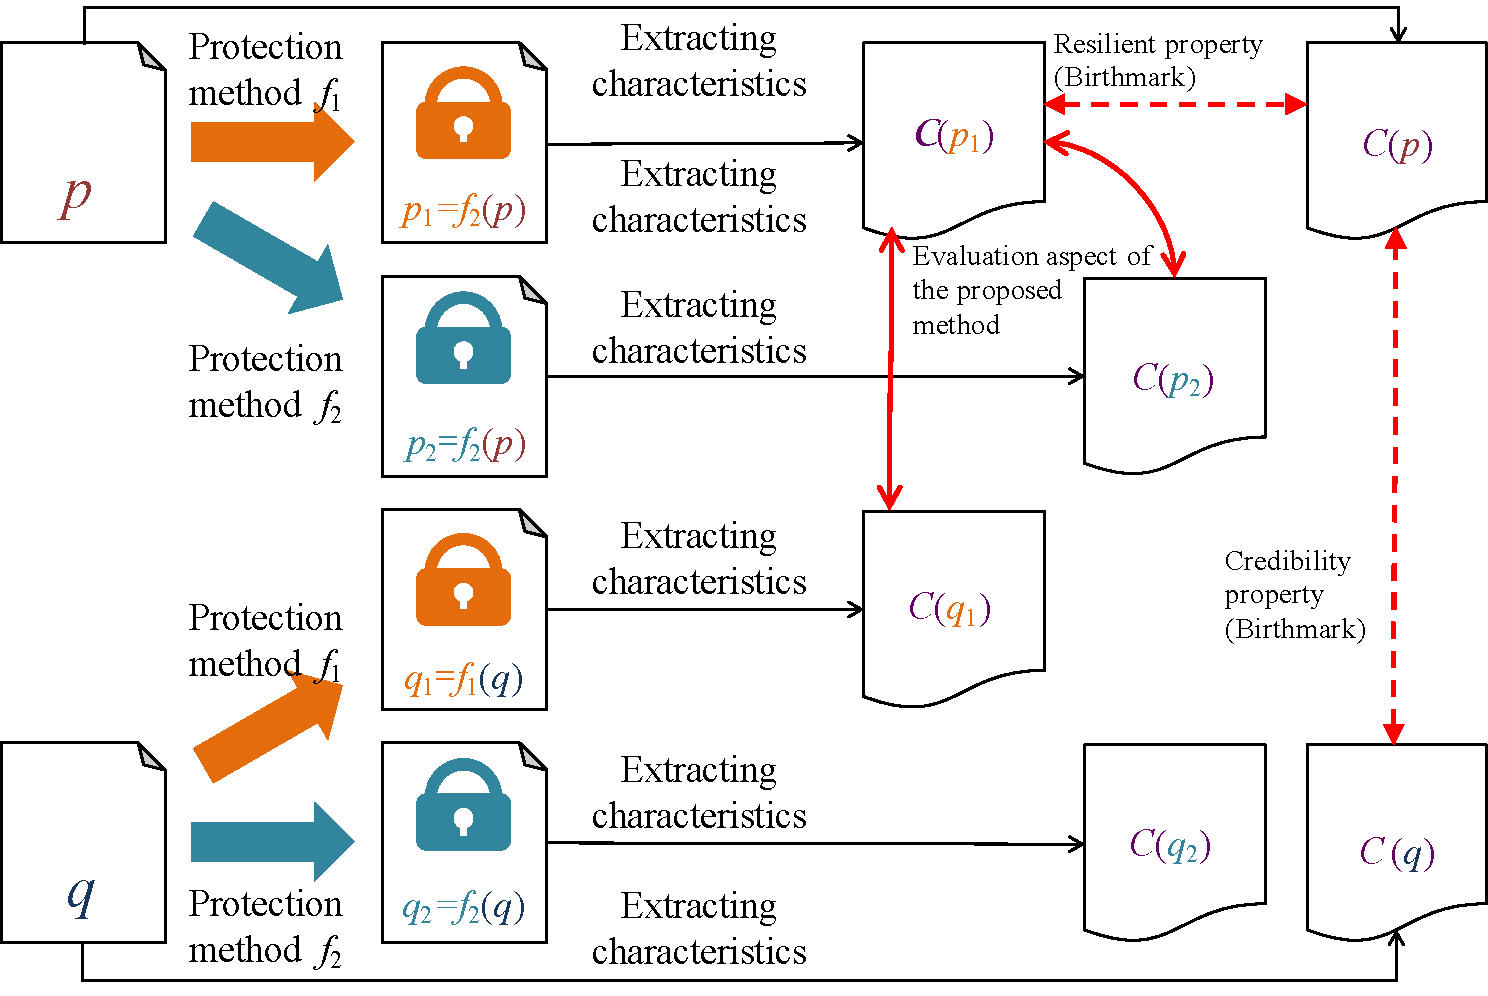
\includegraphics[width=0.78\textwidth]{images/key_idea}
  \caption{提案手法の模式図}\label{fig:keyidea}
\end{figure}

%図\ref{fig:keyidea}に提案手法の模式図を示す

\subsection{characteristic extraction method}
Although Extracting characteristic is like base mark in method,
it do not carry out as expected to itself.
%式が出るので後

Because, different program p and q

\subsection{indication of characteristic}
In the proposed method, we measure the characteristic of method of protection how n-gram of opcode before and after in method of protection were changed.
Thus, we measure four indications how n-gram was changed.

%式が出るので後

First,

%%%前回の予備実験のセクション
%\section{preliminary experiment}
%\subsection{summary}
%Before performing the evaluation experiment, we carry out preliminary experiment.
%
%This purpose is confirmation that is to detect appearing characteristic in method of protection by proposed method.
%Therefore, it obfuscate jar file p,q,r in really for using the obfuscation tool as target to Java.
%
%%式が出るので後
%This method of obfuscation is correspond to fn
%
%
%\subsection{Comparison by the proposed indication}
%
%
%\subsection{histogram in n-gram of opcode}
%
%\subsection{perplexity in n-gram of opcode}
%
%\subsection{analysis in extracted n-gram}


\section{evaluation experiment}
\subsection{summary}
Some characteristic in method of protection have become clear by preliminary experiment.
This purpose is how to decide the method of protection from extracted characteristic.
As extracting characteristic is based on n-gram of opcode such as 
chapter three, verse 2, 
we compare its with perplexity and frequency.

we conducted a preliminary study to investigate the following questions.
RQ1: What kind of characteristic in method of obfuscation? 

RQ2-1:Is the characteristic effective measure for unknown product?

RQ2-2:Is the characteristic effective measure for unknown obfuscation?

\begin{table}[t]
  \centering
  \footnotesize{
    \caption{利用したJarファイル一覧}\label{table:jars}
  \begin{tabular}{l|r||l|r||l|r}
    Product & Version & Product & Version & Products & Version \\ \hline
    ASM       & 3.3.1 & FakeHack  & 1.0 &JCalendar & 1.3.3   \\
    Jhstop    & 0.0.1 & Jwhich    & 1.0   & Robocode-setup & 1.6.0.1 
  \end{tabular}
  \caption{利用した難読化ツール}\label{table:tools}
  \begin{tabular}{ll|l}
      Tools & Abbr. & Overview \\ \hline
      Allatori Java Obfuscator & ALL & 商用の難読化ツール \\ \hline
      ProGurad                 & PG & OSSの難読化ツール \\ \hline
      Sandmark                 & & 研究用の難読化ツール \\
      \hspace{0.2cm} Duplication registers & DR & 代入を重複させる。\\
      \hspace{0.2cm} Merge local integers & MLI & 2つのint変数をlongに収める。\\
      \hspace{0.2cm} Irreducibility       & IRR & 制御フローを複雑にする。\\
  \end{tabular}}
\end{table}

\subsection{analysis in n-gram}
In this purpose, we analyzed order in n-gram by referring to frequency and perplexity in each method of obfuscation.
In the analysis result, It see different order before and after protection in method of obfuscation.

As a result, we analyze the RQ1.

Also, we understand that added order is high value of perplexity and rare order.
For these data, added order
As characteristic in method of obfuscation is added order by these datas, the characteristic are reported TABLE\ref{table:features}.



\begin{table}[t]
  \centering
  \footnotesize{
    \caption{ツールごとの特徴}\label{table:features}
  \begin{tabular}{l|l}
    ツール              & 特徴 \\ \hline
    ALL & オリジナルの命令列を\texttt{swap}命令で入れ替える \\
    PG  & オリジナルと変化なし \\
    DR  & \texttt{istore}命令を2回続けて実行する \\
    MLI & \texttt{dup2x2 lxor}を連続して実行する \\
    IRR & \texttt{nop}命令がある \\
  \end{tabular}}
\end{table}


\subsection{identifying method of obfuscation in known}
In this purpose, unknown product are obfuscated by using the tools in TABLE\ref{table:features}, after we identify how method of obfuscation are used.

As a result, we analyze the RQ2-1.

Not appearing n-gram are researched by n-gram that is before applied obfuscation.
In the result, n-gram of high frequency in five is reported TABLE\ref{table:junit}.
In showing the TABLE\ref{table:junit}, the order are called high value in perplexity such as dup2X2 lxor.
As the order is characteristic, we compare it with characteristic in five tool ( TABLE\ref{table:junit} ).
As a result, characteristic in applied method of obfuscation correspond with characteristic in method of MLI.

\begin{table}[t]
  \centering
  \footnotesize{
    \caption{JUnit (5-gram)の命令列}\label{table:junit}
  \begin{tabular}{l|r|r}
    命令列 & 頻度 & PPL\\ \hline
 %   \multicolumn{1}{p{1cm}}{ORI} & 
 %   \multicolumn{1}{p{1cm}}{ALL} & 
 %   \multicolumn{1}{p{1cm}}{DR} & 
 %   \multicolumn{1}{p{1cm}}{IRR} & 
 %   \multicolumn{1}{p{1cm}}{MLI} & 
 %   \multicolumn{1}{p{1cm}}{PG} & 
 %   \multicolumn{1}{p{1cm}}{PPL} \\ \hline
    \texttt{dup2x2 lxor lconst\_1 lneg bipush}   & 16 & 11.30E+05 \\
    \texttt{lload dup2x2 lxor lconst\_1 lneg}    & 16 &   5.37E+05 \\
    \texttt{bipush lushr land lxor lstore}       &  9 &   0.52E+05 \\
    \texttt{lconst\_1 leng bipush lushr land}    &  9 &   0.96E+05 \\
    \texttt{lneg bipush lushr land lxor}         &  9 &  1.37E+05 \\
  \end{tabular}}
\end{table}

\subsection{identifying method of obfuscation in unknown}
In this purpose, known products are obfuscated by using the unknown method of obfuscation, after we identify how method of obfuscation are used.

As a result, we analyze the RQ2-2.

Not appearing n-gram are researched by n-gram that is before applied obfuscation.
In the result, n-gram of high frequency in five is reported TABLE\ref{table:jhstop}.
In showing the TABLE\ref{table:jhstop}, the order that is high value in perplexity are called dup and imul orders in continuous.
As the order is characteristic, we compare it with characteristic in five tool ( TABLE\ref{table:jhstop} ).
As a result, characteristic in unknown method of obfuscation do not correspond with characteristic in analyzed method.

In the next, as difference product are obfuscated unknown method of obfuscation, we compare the each characteristic.
As a result, as the same characteristic are identified, we understand that unknown method of product is method of SOP.


\begin{table}[t]
  \centering
  \footnotesize{
    \caption{Jhstop (5-gram)の命令列}\label{table:jhstop}
  \begin{tabular}{l|r|r}
   命令列 & 頻度 & PPL\\ \hline
 %   \multicolumn{1}{p{1cm}}{ORI} & 
 %   \multicolumn{1}{p{1cm}}{ALL} & 
 %   \multicolumn{1}{p{1cm}}{DR} & 
 %   \multicolumn{1}{p{1cm}}{IRR} & 
 %   \multicolumn{1}{p{1cm}}{MLI} & 
 %   \multicolumn{1}{p{1cm}}{PG} & 
 %   \multicolumn{1}{p{1cm}}{PPL} \\ \hline  
    \texttt{irem iconst\_0 if\_icmpne aload getfield} & 15 &   0.15E+05 \\
    \texttt{dup dup dup imul imul}                    & 14 &  42.40E+05 \\
    \texttt{dup dup imul imul isub}                   & 14 &   8.74E+05 \\
    \texttt{dup imul imul isub iconst\_3}             & 14 &   3.49E+05 \\
    \texttt{iload dup dup dup imul}                   & 14 & 101.00E+05 \\
    \end{tabular}}
\end{table}


\section{Conclusion}
In this paper, we took the identification of method of protection by watching the unnatural evaluation.
The actual program was applied method of protection and extracted characteristic to base on frequency and perplexity to order line of n-gram.
In this evaluation experiment, the identification of known obfuscation is easy and the identification of unknown obfuscation is difficult.
This solution plan is to increase the characteristic of method of obfuscation.
it can respond to method of unknown obfuscation by increasing characteristic. 


% conference papers do not normally have an appendix


% use section* for acknowledgment
\section*{Acknowledgment}


The authors would like to thank...





% trigger a \newpage just before the given reference
% number - used to balance the columns on the last page
% adjust value as needed - may need to be readjusted if
% the document is modified later
%\IEEEtriggeratref{8}
% The "triggered" command can be changed if desired:
%\IEEEtriggercmd{\enlargethispage{-5in}}

% references section

% can use a bibliography generated by BibTeX as a .bbl file
% BibTeX documentation can be easily obtained at:
% http://mirror.ctan.org/biblio/bibtex/contrib/doc/
% The IEEEtran BibTeX style support page is at:
% http://www.michaelshell.org/tex/ieeetran/bibtex/
\bibliographystyle{IEEEtran}
% argument is your BibTeX string definitions and bibliography database(s)
\bibliography{icis2016_sagisaka}
%
% <OR> manually copy in the resultant .bbl file
% set second argument of \begin to the number of references
% (used to reserve space for the reference number labels box)
%\begin{thebibliography}{1}
%
%\bibitem{IEEEhowto:kopka}
%H.~Kopka and P.~W. Daly, \emph{A Guide to \LaTeX}, 3rd~ed.\hskip 1em plus
%  0.5em minus 0.4em\relax Harlow, England: Addison-Wesley, 1999.
%
%\end{thebibliography}




% that's all folks
\end{document}


